%%=============================================================================
%% Inleiding
%%=============================================================================

\chapter{Inleiding}
\label{ch:inleiding}

Wat is blockchain? Blockchain is een technologie die het best kan vergeleken worden met een database. Het wordt dan ook vooral gebruikt om gevoelige data veilig op te slaan. Blockchain dook voor het eerst op in het Bitcoin whitepaper door \textcite{Nakamoto2008}, dit blijkt een alias te zijn voor een persoon of een groep en de echte ontwikkelaar is niet gekend bij naam. Uit dit document kan afgeleid worden dat het gaat om een enkel persoon maar dit is niet met zekerheid geweten.

Blockchain is meteen ook de technologie achter het bekende Bitcoin. Het idee was om digitaal geld te kunnen transporteren van één partij naar een andere zonder de tussenkomst van een financiële instelling. Blockchain heeft dan ook het grote voordeel te werken met een peer-to-peer systeem wat waarschijnlijk raar klinkt voor een geld transport systeem aangezien banken werkten met een centraal systeem om veiligheid te garanderen. Dit heeft uiteraard ook vele nadelen zoals het integreren met andere platformen. Toch blijkt blockchain een veilige manier te zijn en dit door de manier van hoe blockchain werkt.

\section{Stand van zaken}
\label{sec:stand-van-zaken}

%% TODO: deze sectie (die je kan opsplitsen in verschillende secties) bevat je
%% literatuurstudie. Vergeet niet telkens je bronnen te vermelden!

\subsection{Blockchain}
\subsubsection{Inleiding}
 Blockchain is een peer-to-peer technologie of ook ``ledgers'' genoemd. Dit wil zeggen dat alle data niet in één plaats is opgeslagen maar op verschillende servers of ook nodes genoemd. Zo heeft elke node een versie van de blockchain. Dit is meteen ook één van de reden waarom blockchain zo veilig is en ook niet eenvoudig is om te hacken, bovendien is de blockchain volledig geëncodeerd door middel van een hash. Een voorbeeld van de hash is te zien in op figuur \ref{fig:blockchain-hash-example}. Hoe veilig deze technologie juist is komen we later op terug.
 
 Je kan blockchain het makkelijkst voorstellen als een excel-blad. Elke rij in het blad is een transactie, en de transactie heeft telkens een relatie met de vorige transactie. Dit is te zien op figuur \ref{fig:blockchain-transaction-example}. Zo kan er dus bijvoorbeeld geen 10.000 euro getoverd worden op een bitcoin rekening aangezien deze moet gestort worden met een transactie en dus wel degelijk ergens vandaan moet komen.
 
 \begin{figure}
 	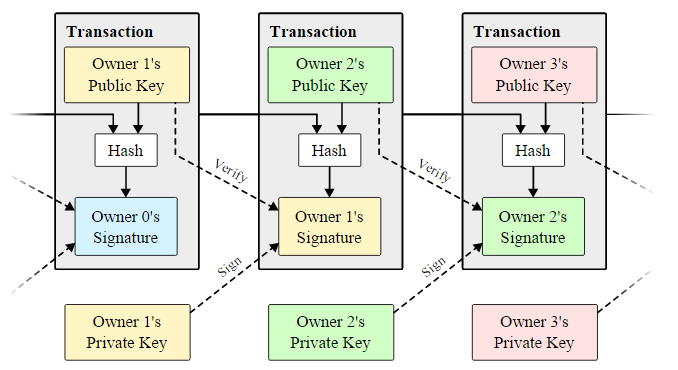
\includegraphics[width=\linewidth]{blockchaintransactions.png}
 	\caption{Voorbeeld van transacties. Bron: Bitcoin.org/bitcoin.pdf}
 	\label{fig:blockchain-transaction-example}
 \end{figure}
\begin{figure}
	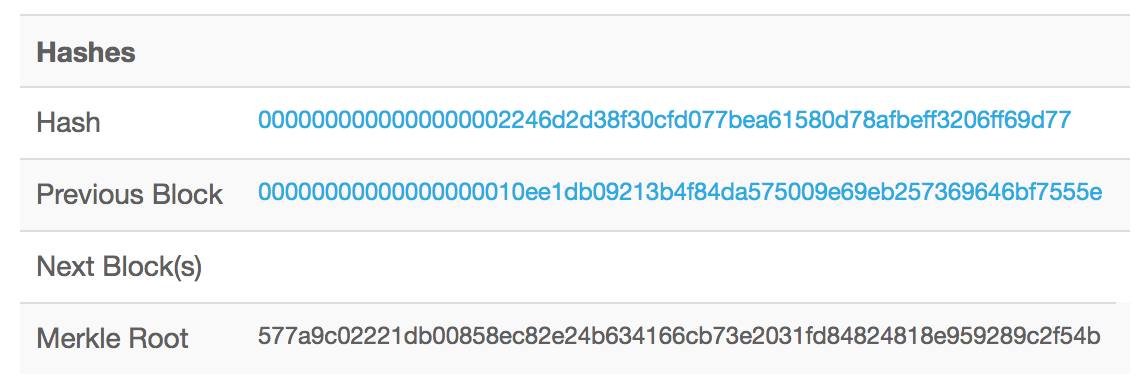
\includegraphics[width=\linewidth]{blockchain-hashes.png}
	\caption{Voorbeeld van hashes. Bron: https://blockchain.info/}
	\label{fig:blockchain-hash-example}
\end{figure}
 
 \subsubsection{Initaliseren van een blockchain}
 Natuurlijk moet er wel een manier zijn om bijvoorbeeld nieuw geld in de blockchain toe te voegen, dit moet dan uiteraard wel ergens vandaan komen dus er moet natuurlijk wel een manier zijn om instanties aan te kunnen maken. 
 
 De eerste transactie in een blok wordt gezien als een speciale transactie die meteen ook een nieuwe munt zal aanmaken waar hij eigenaar van is. Dus voor elke eerste transactie van een blok wordt een nieuwe munt aangemaakt waarvan de node dus eigenaar is. Dit zorgt meteen ook voor een goed motief om het netwerk van nodes te steunen en zorgt ook meteen voor een manier om nieuwe munten in omloop te brengen aangezien er geen centrale authoriteit is die de blockchain beheert. 
 
 Er wordt dus constant geld toegevoegd aan de bitcoin blockchain door het gevolg van het verbruiken van middelen. In het geval van Bitcoin is dit bijvoorbeeld elektriciteit en CPU-kracht en dit zal voor de meeste blockchains ook het geval zijn. Dus met andere woorden wordt het openstellen van CPU-kracht en het gebruik hiervan beloond door het verkrijgen van bitcoins bij het aanmaken van een nieuw blok. Dit heeft ook als voordeel dat het proberen hacken van de blockchain niet meer zo gunstig zou zijn en het dus beter is om een ``eerlijke'' node te blijven. Natuurlijk is het niet nodig om steeds een nieuwe munt aan te maken als motivatie want dit zou zorgen voor inflaties. Wanneer er bijvoorbeeld een genoeg aantal munten in omloop zijn kan het gehele systeem van verbruikte middelen ook vergoed worden door transactiekosten zodat er helemaal geen inflatie optreed.
 
 \subsubsection{Kan iedereen zich aansluiten bij de nodes?}
 Iedereen kan inderdaad lid worden van een blockchain netwerk en CPU-kracht beschikbaar stellen, dit wordt ook ``gold miners'' genoemd. Je stelt je eigen computer ter beschikking als node in het netwerk waardoor jij vergoed wordt met bitcoins. Deze zouden dan ook de kosten moeten dekken van de elektriciteit en de verbruikte CPU-kracht. Wie dus CPU-kracht over heeft kan deze ter beschikking stellen en hier aan verdienen. Op deze manier probeert  bitcoin bijvoorbeeld ook om alle nodes ``eerlijk'' te houden aangezien dit veel interessanter zou zijn. Het opstellen van een gold miner wordt later uitgelegd. 
 
 Tegenwoordig kan je niet meer je eigen computer ter beschikking stellen voor Bitcoin aangezien de verloning voor elektriciteit en CPU-kracht te laag zou zijn om dit competetief te houden. Daarom is er tegenwoordig hardware te koop om Bitcoins te minen die gemaakt zijn speciaal hiervoor. Deze zijn meteen ook veel zuiniger. Dit volgens het volgende artikel \textcite{Bitcoinmining.com}.
 
 \subsubsection{Hoe gebeurd de validatie?}
 Hoe wordt er voorkomen dat er illegale transacties worden uitgevoerd? Het hele systeem werkt aan de hand van peer-to-peer, elke server heeft dus zijn eigen versie. Telkens er een verandering wordt uitgevoerd dan wordt de blockchain verandering gebroadcast over het hele netwerk. Vervolgens gaat elke node die de transactie ontving deze gaan plaatsen in een blok. Elke node zal vervolgens een moeilijke proof-of-work genereren. Wat een proof-of-work juist is wordt uitgelegd in volgend puntje. Wanneer een node een proof-of-work gegenereerd heeft dan zal hij deze block versturen naar alle andere nodes in het netwerk. Vervolgens zullen de nodes het block enkel en alleen aanvaarden als alle transacties in het block kloppen en nog niet vervallen zijn. Om aan te tonen dat een node het block heeft aanvaard zal deze node de hash van deze block gebruiken in de volgende block als vorige hash. 

\begin{figure}
	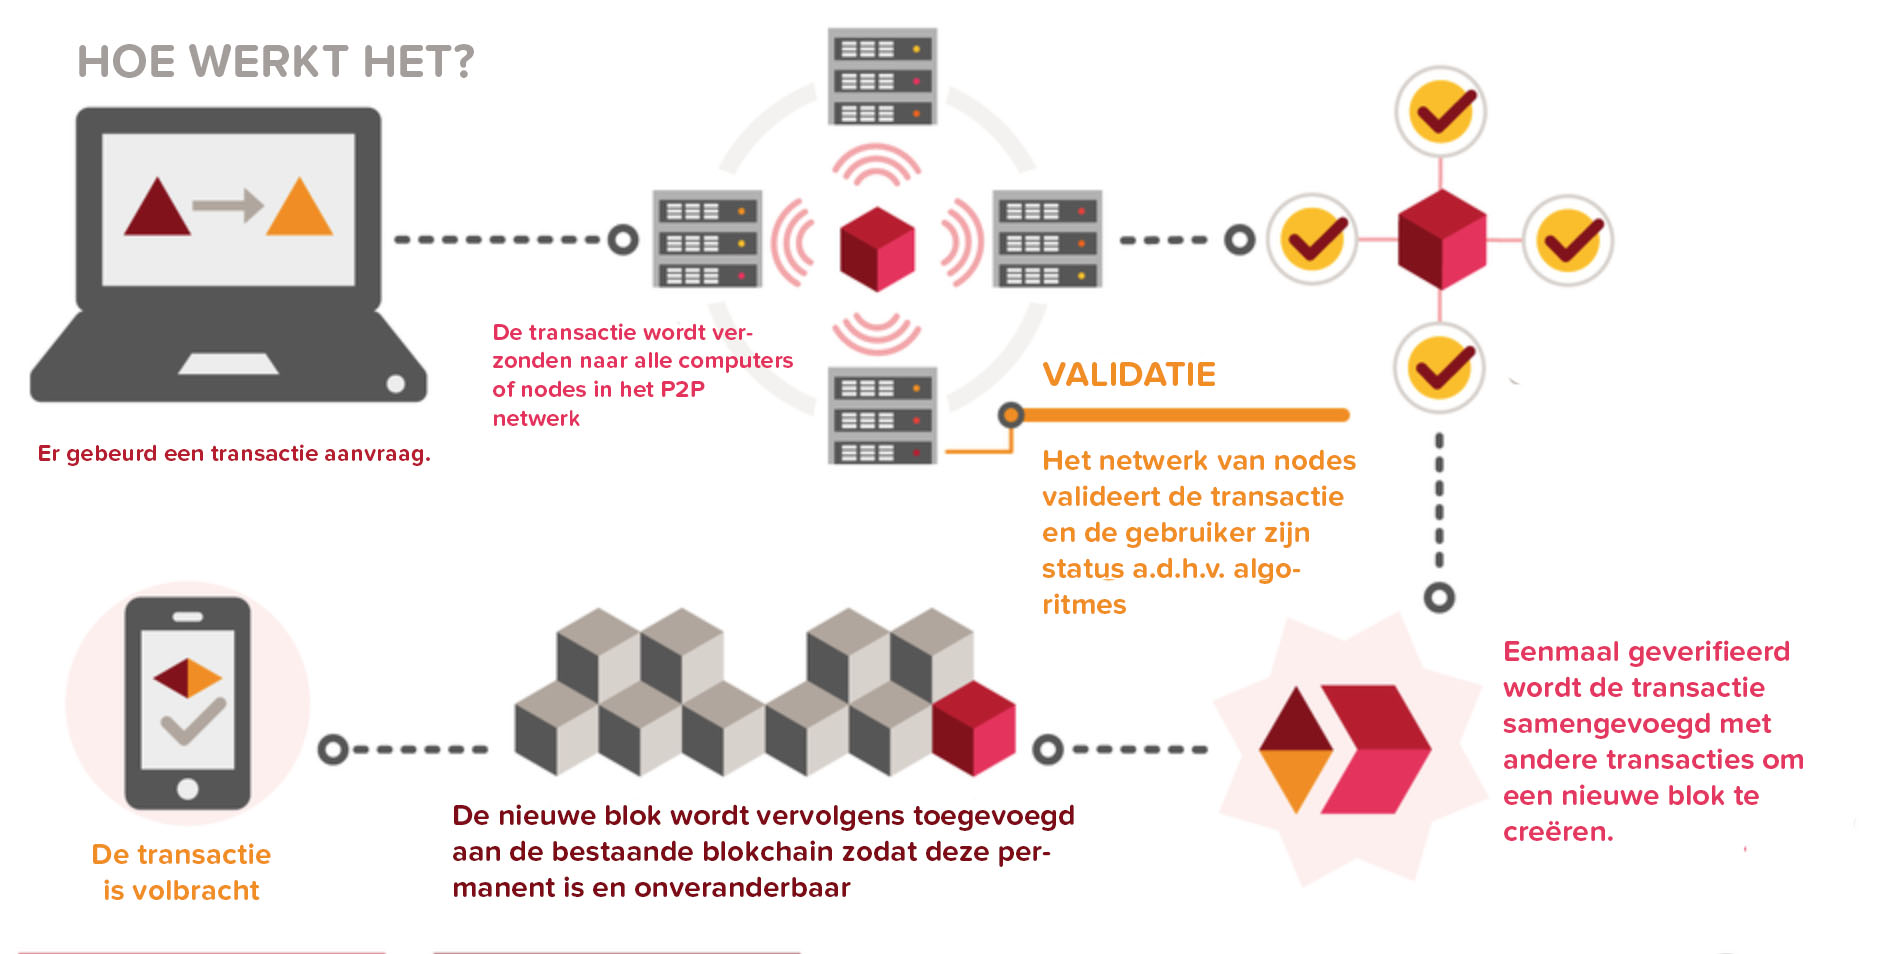
\includegraphics[width=\linewidth]{blockchain-howto.jpg}
	\caption{Grafische voorstelling van de werking van blockchain. Bron: http://usblogs.pwc.com/emerging-technology/wp-content/uploads/2016/11/blockchain-infographic.0.png}
	\label{fig:blockchain-howto}
\end{figure}

In het algemeen zullen de nodes altijd de langste ``ketting'' aanvaarden als de correcte en zal het verder werken aan deze ketting. Wanneer twee nodes een verschillend blok gaan broadcasten dan kan het zijn dat één node de ene versie eerst zal krijgen en een andere de alternatieve versie eerst zal ontvangen. Daarom zal altijd de eerste die ontvangen werd gebruikt worden. De alternatieve versie wordt dan bijgehouden. Deze koppeling wordt onderbroken vanaf er een nieuwe proof-of-work wordt gevonden. Hierdoor zal één van de twee versies langer worden en de langste versie zal dan gebruikt worden om op verder te bouwen. De nodes die ondertussen op de andere tak aan het werken waren zullen dan ook overschakelen op deze. Dit wil natuurlijk niet zeggen dat een transactie broadcast alle nodes moeten bereiken, het blijft steeds het internet en een transactie kan verloren geraken. Dit is geen probleem zolang er maar genoeg nodes de transactie ontvangen en deze verifiëren. De nodes die die transactie niet ontvingen zullen dit merken wanneer ze de volgende blok ontvangen en zien dat ze er één hebben gemist en zal deze dan aanvragen aan de andere nodes in het netwerk. De volledige werking is visueel weergegeven op Figuur \ref{fig:blockchain-howto}

\subsubsection{Wat betekent proof-of-work?}
Proof-of-work is een maatregel die werd ingevoerd om bepaalde aanvallen te voorkomen zoals de gekende denial of service of ook DOS-aanvallen genoemd of om spam op een netwerk tegen te gaan en dit door werk te vragen van de service aanvrager meestal in de vorm van verwerkingstijd door een computer. Proof-of-work kan voorkomen in verschillende vormen, meestal zijn dit wiskundige algoritmen. Enkele voorbeelden zijn puzzels, Diffie-Hellman puzzels, hash sequencies, Merkle tree gebaseerde algoritmen en nog enkele meer. 

Verder zijn er ook verschillende varianten. Deze zijn de Challenge-response en Solution-verification. Het verschil tussen beide kort samengevat komt neer op het volgende, bij challenge-response is de taak die moet uitgevoerd worden nog niet bekend. De server zal deze sturen bij het aanvragen van een service. Bij Solution-verification is de taak op voorhand gekend en kan deze meteen meegestuurd worden met de request. Deze informatie is terug te vinden op  \textcite{Wikipedia-POW}. Een grafische voorstelling van beide is te vinden op Figuur \ref{fig:pow-challengeresponse} en Figuur \ref{fig:pow-solutionverification}. De proof-of-work die Bitcoin zelf gebruikt is bijvoorbeeld gebaseerd op Adam Back's Hashcash, dit volgens \textcite{Nakamoto2008}.

\begin{figure}
	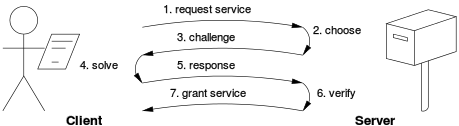
\includegraphics[width=\linewidth]{pow-challengeresponse.png}
	\caption{Grafische voorstelling van de werking van challenge response. Bron: en.wikipedia.org/wiki/Proof-of-work\_system}
	\label{fig:pow-challengeresponse}
\end{figure}

\begin{figure}
	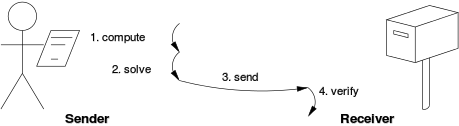
\includegraphics[width=\linewidth]{pow-soultionverification.png}
	\caption{Grafische voorstelling van de werking van solution verification. Bron: en.wikipedia.org/wiki/Proof-of-work\_system}
	\label{fig:pow-solutionverification}
\end{figure}

\subsubsection{Hoe veilig is blockchain?}
\label{sec:hoeveiligisblockchain}
Wanneer er dus een aanval gebeurt op de blockchain of dus een illegale transactie plaats vindt dan kan deze verworpen worden door de andere servers. In simpele termen komt het er op neer dat zolang de totale CPU capaciteit van de servers groter is dan de capaciteit van de aanvaller dat de blockchain dus veilig is en de aanvallen zal afweren. Dit omdat de aanvaller sneller een alternatieve ketting zou moeten produceren  dan dat de vertrouwde nodes dit doen. Zelf in het geval dat dit zou gebeuren wil dit niet zeggen dat de vertrouwde nodes dit zullen accepteren aangezien dat de aanvaller ook geen waarde kan creëren uit het niets of zichzelf eigenaar kan maken van andere waarden als we dit zouden bekijken in het systeem van Bitcoins. Het enige wat een aanvaller dus in principe kan doen is het aanpassen van zijn eigen transacties, bijvoorbeeld dus geld terug nemen dat hij al eerder uitgaf. De kans dat zich dit voordoet is uitermate klein. Zo is te zien in de whitepaper van \textcite{Nakamoto2008}. Stel dat de aanvaller 10 blokken achter zit en de vertrouwde ketting moet inhalen dan heeft deze een kans van 0.0000012\% wanneer we er vanuit gaan dat de aanvaller 10 \% kans heeft om de volgende blok te vinden. Verdere berekeningen zijn te vinden in de paper van \autocite{Nakamoto2008}.


\subsubsection{Andere soorten ``hacks''}
Er zijn uiteraard verschillende manieren van ``hacken'', één van de bekendste is bitcoin mining malware. Dit is malware die verspreid wordt en computers en apparaten infecteerd. De geïnfecteerde apparaten worden hierdoor gebruikt om bitcoins te minen wat de toestellen uiteraard zwaar vertragen. 

Andere zaken die veel voorkomen zijn het hacken van de bitcoin wallets, dit zijn bestanden die op de machine staan en die de bitcoins bij houd. Deze ``wallets'' bevinden zich op de hardeschijf en kunnen dus gestolen worden. 

Trojans zijn ook bij bitcoin een plaag. Zo zijn er trojans die slechts activeren wanneer er een crypto-currency nummer wordt ontvangen en die deze dan manipuleren zodat de gebruiker bijvoorbeeld geld overschrijft naar de verkeerde persoon. 

Verder zijn er ook nog fouten in de software die bijvoorbeeld toegang geeft tot een blockchain. Blockchain mag in theorie en praktijk nog zo veilig zijn, als er software gebruikt wordt die malfunctioneert dan kan de veiligheid van blockchain ook snel te niet gedaan worden.

Zoals eerder vermeld zijn de transacties of sommige zaken versleuteld voor het publiek. De transactie zelf is zichtbaar maar sommige zaken zijn versleuteld. Wanneer deze encryptie bijvoorbeeld niet sterk genoeg is kan het zijn dat hackers een bepaald deel van de versleutelde tekst toch kan ontfutselen. Blockchain gebruikt in het algemeen een SHA-256 versleuteling, deze word onder andere ook gebruikt voor het versleutelen van HTTPS en dergelijke. Wanneer deze encryptie zou falen zou niet enkel blockchain dus een zwaar probleem hebben. Onderzoekers bevestigden wel dat SHA-256 zeker sterk genoeg is om zaken te beveiligen voor een hele tijd.

\subsubsection{Wat is SHA-256}
SHA-2 is een verzameling van cryptografische hash functies die gemaakt werden door de National Security Agency (NSA). Wat zijn cryptografische hash functies? Dit zijn wiskundige bewerkingen die kunnen uitgevoerd worden op digitale data. Door vervolgens de berekende ``hash'' te vergelijken met de verwachte hash kan men de data integriteit bepalen. Om een voorbeeld te geven om dit principe te verduidelijken nemen we het volgende voorbeeld. We hebben een bestand gedownload, laat ons zeggen dat dit een ``word'' bestand is. We maken een kopie van dit bestand en passen in het word document enkele dingen aan. We slaan vervolgens het document op en berekenen de hash van beide documenten. Nu hebben we dus het originele bestand en het aangepaste bestand. Als we nu de hash zouden vergelijken van beide documenten dan gaan we zien dat deze verschillen. Mochten we nu van de originele versie nog een kopie maken en hiervan de hash berekenen dan zal deze dezelfde zijn van het originele bestand. Op deze manier kunnen we dus bekijken of een bestand gewijzigd is of niet. Een grafisch voorbeeld van dit voorbeeld is te zien in Figuur \ref{fig:hash-example}.

 \begin{figure}
 	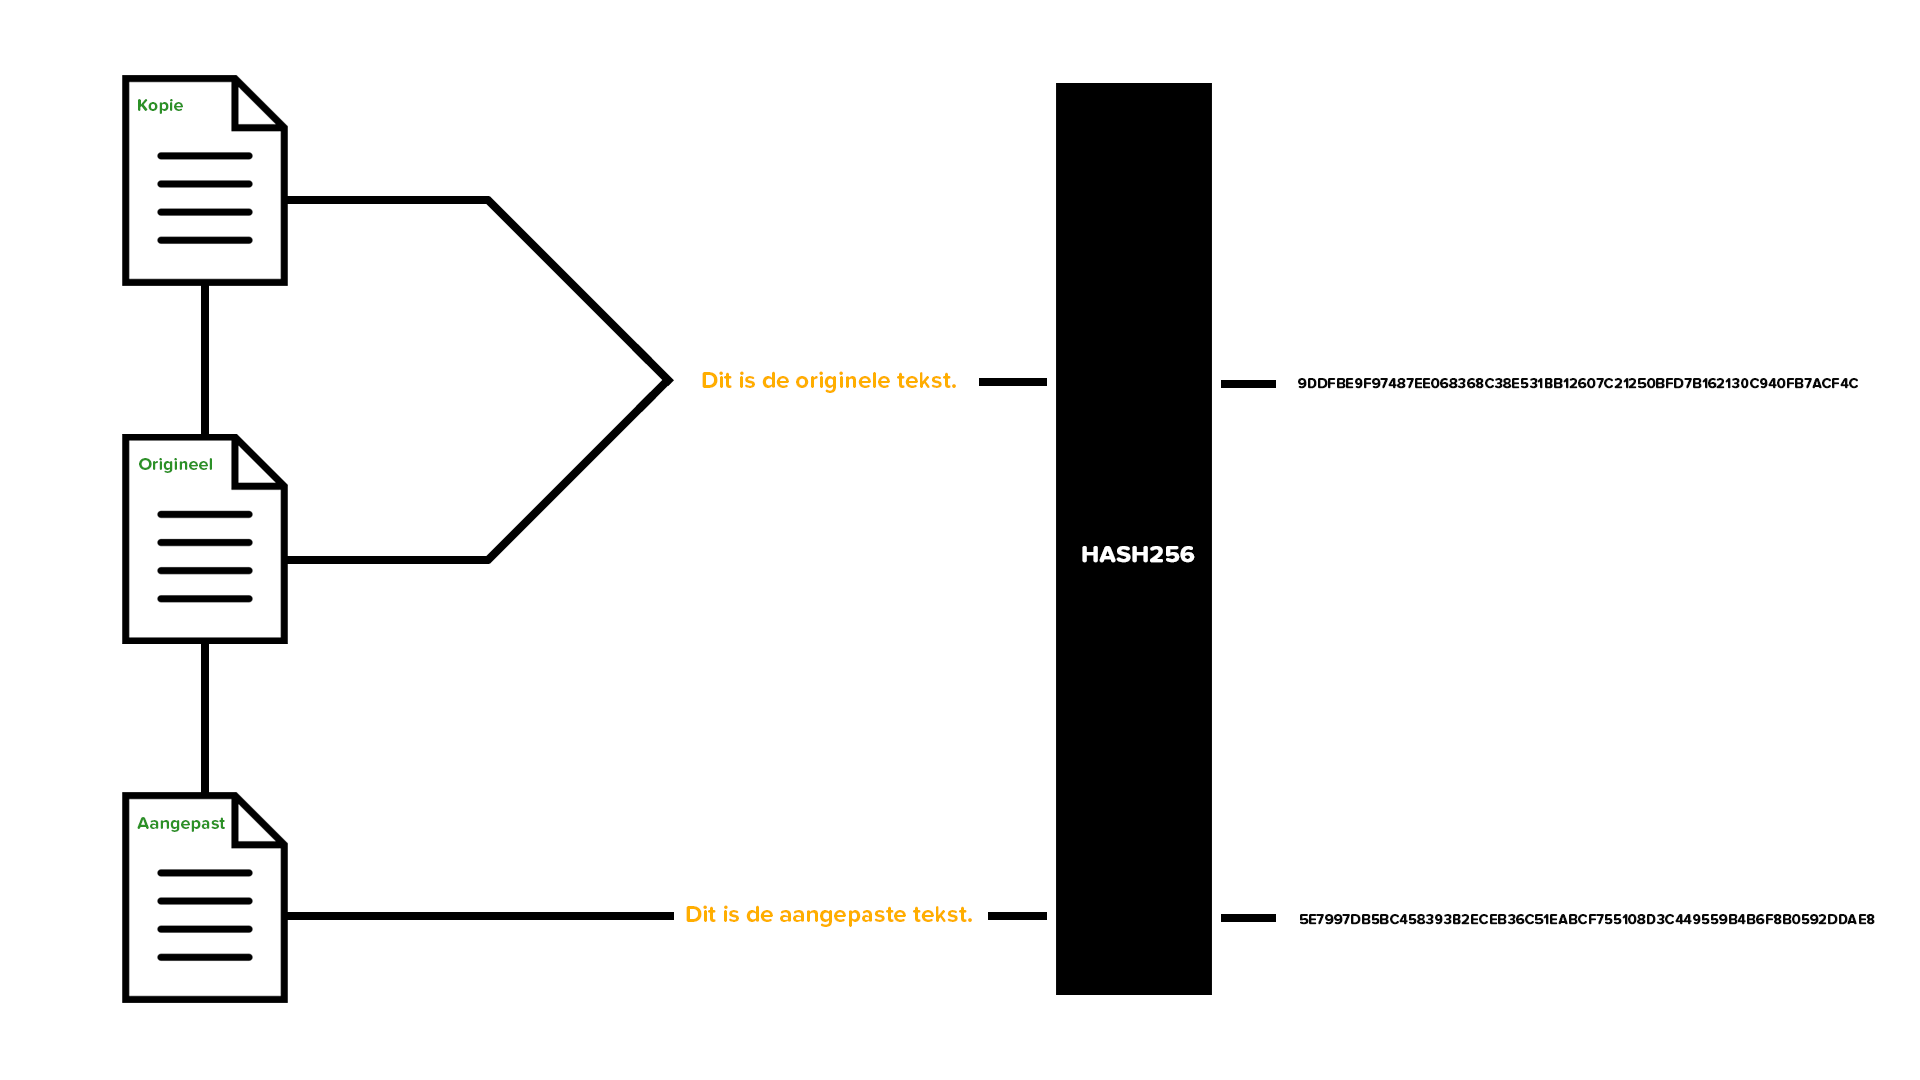
\includegraphics[width=\linewidth]{hash-example.png}
 	\caption{Grafische voorstelling van de werking van sha256.}
 	\label{fig:hash-example}
 \end{figure}



\subsection{Verzekeringen en unieke documenten}
\subsubsection{Wat is een verzekeringsagent en een verzekeringsmakelaar?}
Een verzekeringsagent is een gebonden tussenpersoon. Dit wil zeggen dat deze persoon voor één verzekeringsmaatschapij werkt, dit verschillend van een verzekeringsmakelaar die onafhankelijk is en niet gebonden is aan één verzekeringsmaatschapij. Een verzekeringsagent kan dus slechts de verzekeringen aanbieden van zijn eigen maatschapij waar een verzekeringsmakelaar verzekeringen kan aanbieden van verschillende maatschapijen. 

Er zijn uiteraard meerdere benamingen voor een verzekeringsagent die allemaal op hetzelfde neerkomen zo wordt een verzekeringsagent bijvoorbeeld ook een tussenpersoon genoemd, een intermediair of een financieel adviseur. 

\subsubsection{Wat doet een verzekeringsagent of verzekeringsmakelaar?}
Zoals eerder vermeld doet een verzekeringsagent en verzekeringsmakelaar juist hetzelfde. Het enige verschil tussen beide is dus dat een verzekeringsagent gebonden is aan één maatschapij waar een verzekeringsmakelaar dit niet is. Voor vereenvoudiging doorheen dit document zal ik steeds verwijzen naar een verzekeringsmakelaar. 

Wat doet een verzekeringsmakelaar nu juist? Een verzekeringsmakelaar zal jouw wensen en vragen allemaal noteren en zal dit gebruiken om de voor u zo optimale verzekering te vinden. Nadien overloopt deze dan alle mogelijkheden met de nodige uitleg. Verzekeren kan een zeer complex iets zijn en dan is een verzekeringsmakelaar zeker nuttig om te raadplegen. Dit alles is te vinden in volgend document \textcite{Verzekeruzelf.nl}.

\subsubsection{Soorten verzekeringen en verzekeringsdocumenten}
Er zijn heel veel soorten verzekeringen. Zo kan in theorie alles verzekerd worden al is dit niet altijd gebruikelijk. In volgend document \textcite{verzekeringen.com2015} vind je alvast enkele voorbeelden van beroemdheden die verschillende lichaamsdelen lieten verzekeren want ook dit is uiteraard mogelijk. Bijvoorbeeld wanneer een gitarist zijn hand zou verliezen dan verliest deze hiermee ook meteen de mogelijkheid tot het uitoefenen van zijn beroep. Er zijn dus heel wat mogelijkheden beschikbaar, volgens het volgende artikel \textcite{BFOverzekeringen} van de Belgische overheid zijn dit de meest voorkomende verzekeringen.

\begin{itemize}
	\item Autoverzekering
	\item Brandverzekering en natuurrampen
	\item Familiale BA-verzekering
	\item Rechtsbijstand
	\item Ziekte- en hospitalisatieverzekering
	\item Reisverzekering
	\item Vrijwilligersverzekering
	\item Schuldsaldoverzekering
	\item Levensverzekering of overlijdensverzekering
	\item Verzekeringen in specifieke situaties
\end{itemize}

Voor elk van bovenstaande verzekeringen is er dus een contract, dit bijgevolge ook uniek zal zijn en bepaalde voorwaarden zal bevatten. Documenten zoals deze zouden dus perfect in een blockchain kunnen opgeslagen kunnen worden. 

\subsubsection{Is verzekeren verplicht?}
Er wordt inderdaad ook onderscheid gemaakt tussen verplichte verzekeringen en niet verplichte verzekeringen. Zo kan je verplicht zijn een verzekering te nemen om een bepaalde activiteit te mogen uitvoeren. Denk maar aan een BA verzekering, wanneer je wagen niet verzekerd is dan kan deze niet in verkeer worden gebracht. Daar tegenover is een bestuurdersverzekering geen verplichte verzekering. Ook voor het uitvoeren van bepaalde beroepen is het verplicht om een verzekering aan te gaan. Enkele voorbeelden zijn architecten, boekhouders, belastingsconsulenten en nog vele meer. Sommige verzekeringen kunnen dan weer wel contractueel verplicht worden. Zo kan een huisbaas bijvoorbeeld de huurder verplichten een brandverzekering af te sluiten. Dit volgens het volgende artikel van \textcite{BFOverplichteVerzekeringen}. 

%%\lipsum[7-20]

\section{Probleemstelling en Onderzoeksvragen}
\label{sec:onderzoeksvragen}

%% TODO:
%% Uit je probleemstelling moet duidelijk zijn dat je onderzoek een meerwaarde
%% heeft voor een concrete doelgroep (bv. een bedrijf).
%%
%% Wees zo concreet mogelijk bij het formuleren van je
%% onderzoeksvra(a)g(en). Een onderzoeksvraag is trouwens iets waar nog
%% niemand op dit moment een antwoord heeft (voor zover je kan nagaan).

\section{Opzet van deze bachelorproef}
\label{sec:opzet-bachelorproef}

%% TODO: Het is gebruikelijk aan het einde van de inleiding een overzicht te
%% geven van de opbouw van de rest van de tekst. Deze sectie bevat al een aanzet
%% die je kan aanvullen/aanpassen in functie van je eigen tekst.

De rest van deze bachelorproef is als volgt opgebouwd:

In Hoofdstuk~\ref{ch:methodologie} wordt de methodologie toegelicht en worden de gebruikte onderzoekstechnieken besproken om een antwoord te kunnen formuleren op de onderzoeksvragen.

%% TODO: Vul hier aan voor je eigen hoofstukken, één of twee zinnen per hoofdstuk

In Hoofdstuk~\ref{ch:conclusie}, tenslotte, wordt de conclusie gegeven en een antwoord geformuleerd op de onderzoeksvragen. Daarbij wordt ook een aanzet gegeven voor toekomstig onderzoek binnen dit domein.

